\documentclass[danish]{report}

\usepackage[utf8]{inputenc}
\usepackage[danish]{babel}
\usepackage{listings}
\usepackage{color}
\usepackage{courier}
\usepackage{parskip}
\usepackage{graphicx}
\usepackage{mathtools}
\usepackage{amsfonts}

\definecolor{dkgreen}{rgb}{0,0.6,0}
\definecolor{gray}{rgb}{0.5,0.5,0.5}
\definecolor{mauve}{rgb}{0.58,0,0.82}

\lstset{
  frame=,
  language=C,
  aboveskip=3mm,
  belowskip=3mm,
  showstringspaces=false,
  columns=flexible,
  basicstyle={\small\ttfamily},
  numbers=none,
  numberstyle=\tiny\color{gray},
  keywordstyle=\color{blue},
  commentstyle=\color{dkgreen},
  stringstyle=\color{mauve},
  breaklines=true,
  breakatwhitespace=true
  tabsize=4
}

% Title Page
\title{Obligatorisk opgave 1}
\author{Jacob B. Cholewa \& Mathias Pedersen }


\begin{document}
\maketitle
\chapter{Multitrådet sum}
På en multicore processror kan vi kører til i parallel. Det vil vi i denne opgave udnytte til hurtigere at udregne $ sum = \displaystyle\sum\limits_{i=0}^n \sqrt{i} $.

Først vil vi beskrive hvordan man kører ting i parallel. Vi bruger biblioteket pthread som bruger linux kernes POSIX kald. En tråd har hver sin stack, process nummer, program counter og register, men deler de andre ressourcer i processen med de andre tråde. (se figur \ref{fig:1})


\begin{figure}[H]
\begin{center}
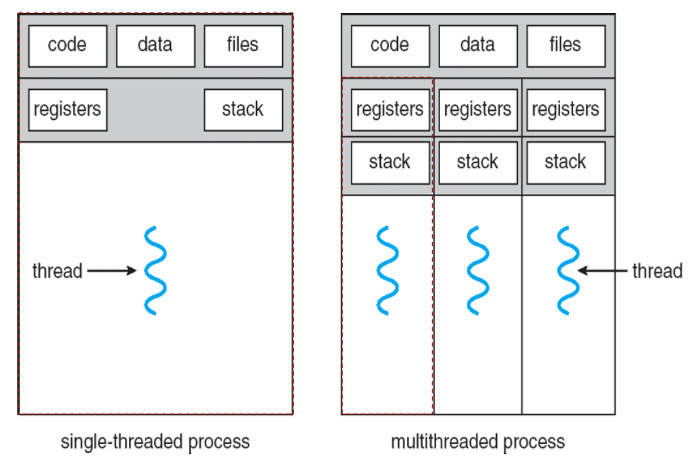
\includegraphics[scale=0.4]{img/1.png}
\caption{Figure der viser enkelt og flertrådede processes}
\label{fig:1}
\end{center}
\end{figure}


Dette gør det nemmere og hurtigere end at oprette en ny process. Hurtigere fordi der ikke skal oprettes lige så meget nyt data og nemmere hvis man har brug for at tilgå den samme data. For at starte en ny tråd kalder vi



\begin{lstlisting}
pthread_create(&tid, NULL, method, args);
\end{lstlisting}

hvor tid er trådens id, NULL bliver sat fordi vi vil køre den med standard indstillinger, method er metoden vi gerne vil køre og args er de argumenter der skal gives til metoden. Metoder der køres skal have typen textit{void *} og argumentet og parmetre skal også have typen \textit{void *}.

For at kunne vente på en tråd bliver færdig, for eksempel hvis vi har brug for et resultat, kan vi bruge 

\begin{lstlisting}
pthread_join(&tid, NULL);
\end{lstlisting}


For at kunne køre udregningen i parallel skal vi kunne opdele beregningen til mindre udregninger der kan køres parallelt og tilsidst så lægges sammen. 

\begin{equation*}
sum = \displaystyle\sum\limits_{i=0}^n \sqrt{i} = \displaystyle\sum\limits_{j=0}^{p} \left( \displaystyle\sum\limits_{i=\frac{j}{p}+1}^{\frac{n}{p}} \sqrt{i} \right), \frac{n}{p} \in \mathbb{N} \text{ hvor } p \text{ lig antallet af tråde}
\end{equation*}


Det har vi gjort med følgende algoritme.

\begin{lstlisting}
int cut, last = 0, threadsleft = nthreads;
for(int i = 0; i < nthreads; i++){
    /* calculates the range that thread i should calculate */
    cut = sumto / threadsleft;
    /* prepares the argument for thread i */
    args[i] = (Runnerargs)  {(last + 1),(last + cut),&sum[i]};

    /* starts a new thread that runs the method runner with arguments args[i] */
    pthread_create(&tid[i],NULL,runner,&args[i]);

    /* removes the range from the amount still needed to be calculated */
    sumto -= cut;

    /* decrement the amount of threads needed to be started */
    threadsleft--;

    /* saves the last element calculated by this thread */
    last+=cut;
}
\end{lstlisting}

Vi deler altså mængden vi skal udregne med antal tråde der mangler at blive startet og trækker den mængden fra den samlede mængde. På den måde sørger vi altid for at udregne hele mængden selvom den ikke kan deles lige med antal tråde. 

Til sidst venter vi på at alle trådene er færdige med at beregne og lægger resultaterne sammen.

\begin{lstlisting}    
double total_sum = 0;
for(int i = 0; i < nthreads; i++){
    pthread_join(tid[i],NULL);
    total_sum += sum[i];
}
\end{lstlisting}

\chapter{Multitrådet FIFO buffer som kædet liste}
\chapter{Producer-Consumer med bounded buffer}
\chapter{Banker’s algorithm til håndtering af deadlock}


\end{document}          
